\documentclass[12pt, a4paper]{article}
\usepackage[utf8]{inputenc}
\usepackage[ngerman]{babel}
\usepackage{csquotes}
\usepackage{pdfpages}
\usepackage{graphicx}
\title{Übungsblatt 5}
\author{Vivien Wallner}
\date{}

\begin{document}
	\maketitle

	\section*{26}
	\subsection*{IP Multicast:}
	Multicast ermöglicht auf der IP Ebene, Daten an eine Empfängergruppe weiter zu senden. Es muss vom Sender  nur einmal versendet werden . Die Daten werden vervielfältigt durch die Router innerhalb des Netzwerks.\\
	Der Multicastdatenverkehr wird nur von jenen Mitgliedern einer Gruppe von Endpunkten verarbeitet, die den Multicastdatenverkehr überwachen (die Multicastgruppe). Alle anderen Knoten ignorieren den Multicastdatenverkehr.
	Eine Gruppe wird durch eine einzelne IP-Multicastadresse identifiziert. Hierbei handelt es sich um eine IP-Adresse im Klasse D-Bereich von 224.0.0.0 bis 239.255.255.255.\\
	Dieses eine versendete Paket, wird nur von Empfängern angenommen, die der entsprechenden IGMP Gruppe angehören.\\


	\subsection*{IGMP}
	
	Internet Group Management Protocol → Protokoll, welches für die Gruppenverwaltung von IP-Multicast verwendet wird. Über IGMP werden von Endgeräten und Routern 
	\begin{itemize}
		\item Join (Gruppenbeitritt) 
		\item Leave (Verlassen einer Gruppe)
		\item Query (Gruppenzugehörigkeitsabfrage)
	\end{itemize}
	versendet oder abgefragt.\\
	Bei Gruppenbeitritt wird dem lokalen Router mitgeteilt, dass das neue Gruppenmittglied an dem Empfang von Paketen des Empfängers interessiert ist.


	\subsection*{Zweck IP Multicast:}

		Es wird verwendet zur effizienten Verbindung zwischen einem Punkt zu mehreren Punkten. Die Daten die von den mehreren Punkten empfangen werden sind alle identisch.

	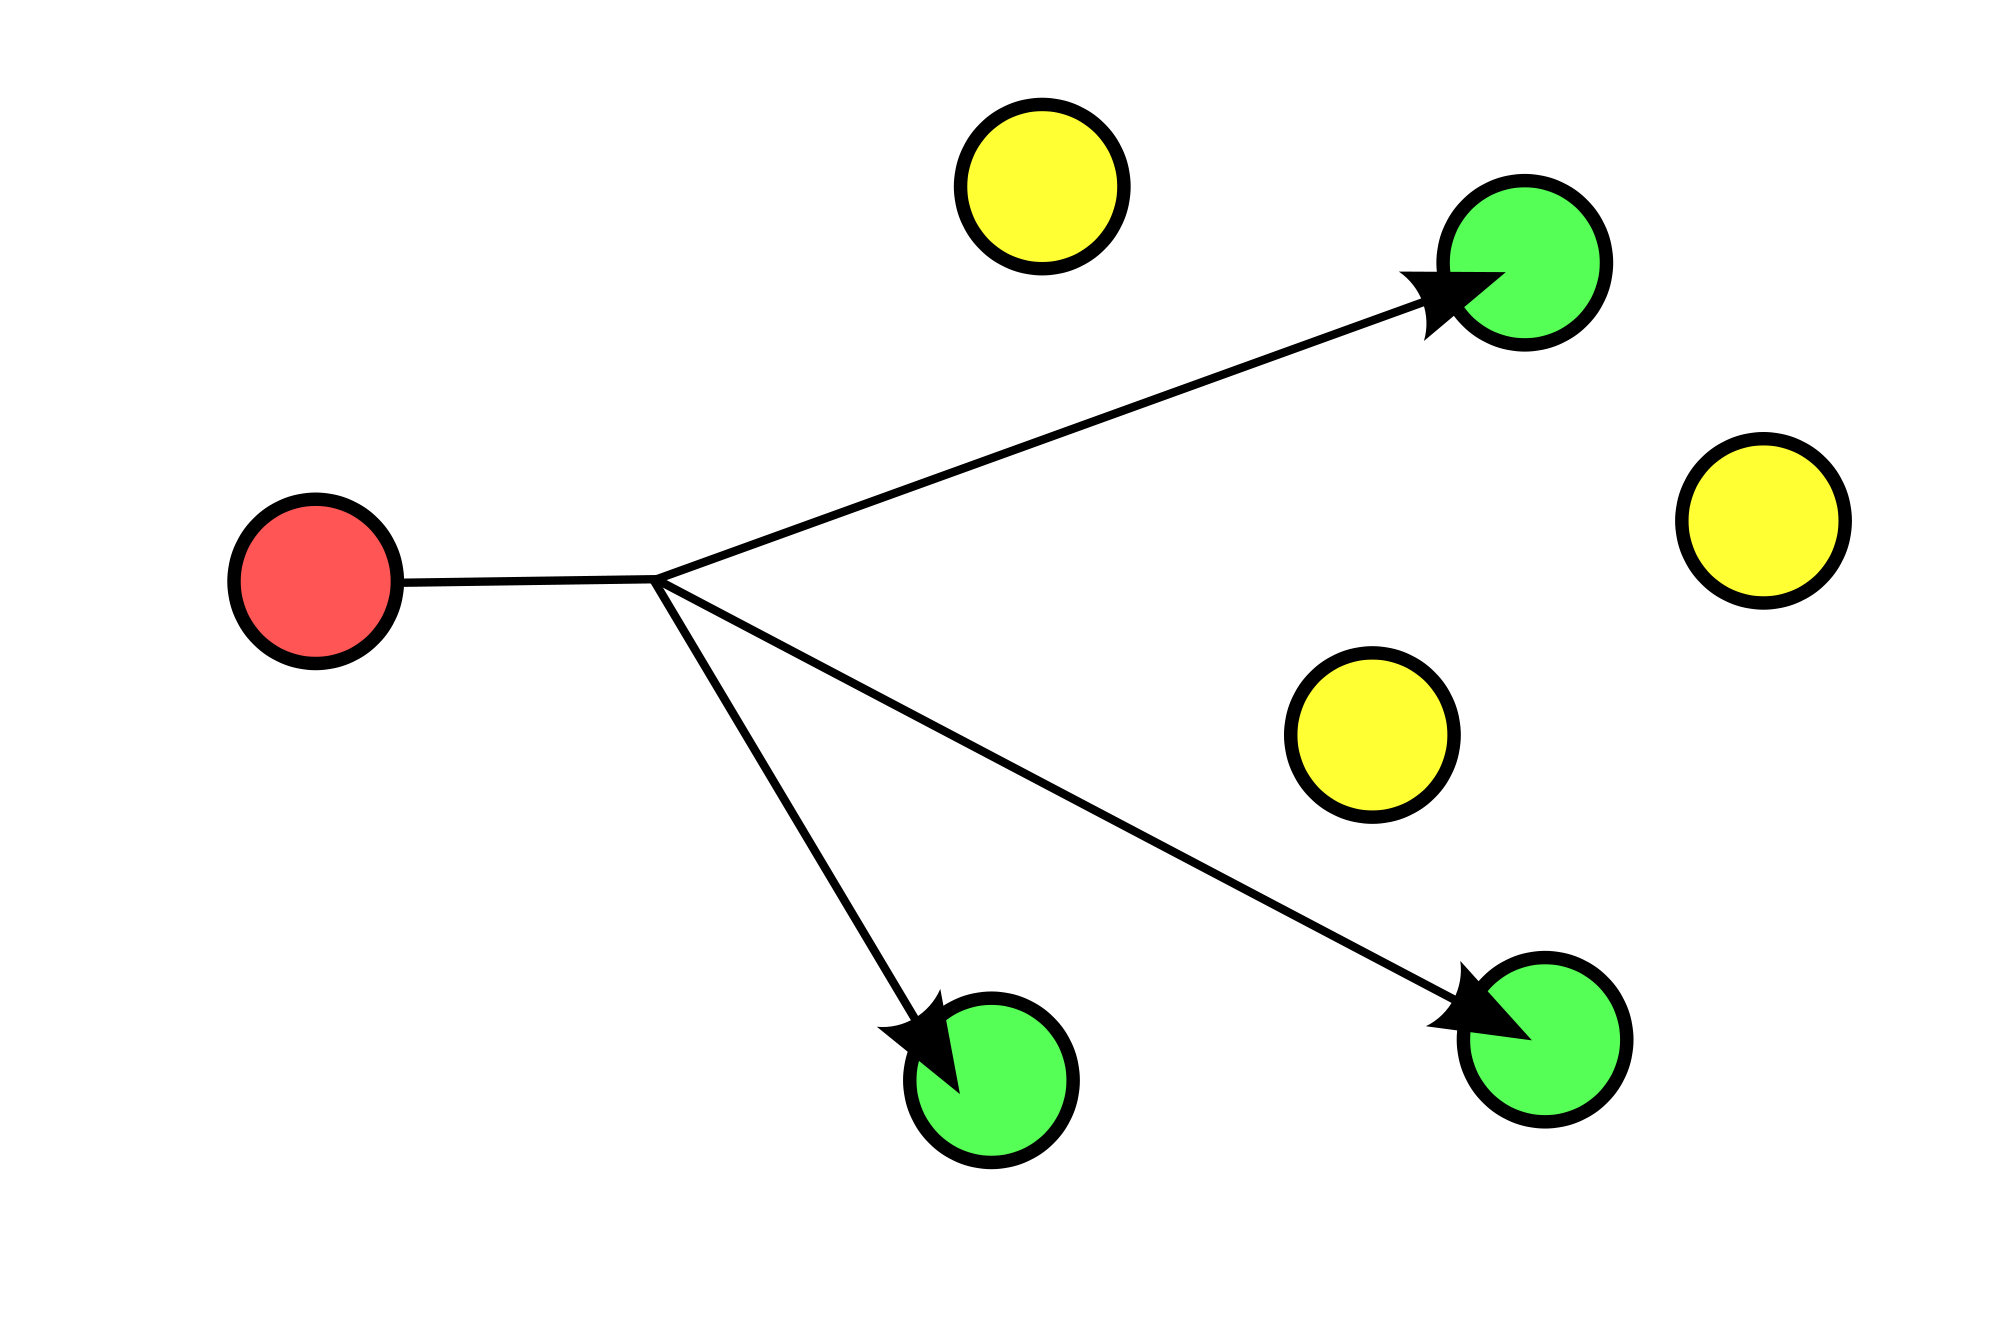
\includegraphics[width=10cm]{multicast.png}\\
	
	Ein Sender sendet identische Daten zu einer großen Anzahl von Empfängern. 
	Bsp: 
	Live-Streaming von Fernseh- oder Radioübertragung

	\subsection*{RFC}
	IP Multicast beschreibt in RFC 1112 (Host Extensions for IP Multicasting), es wurde 1986 Standardisiert.
	Die Spezifikationen wurden argumentiert in RFC 4604 (Using Internet Group Management Protocol Version 3 (IGMPv3) and Multicast Listener Discovery Protocol Version 2 (MLDv2) for Source-Specific Multicast) um Gruppenmanagement zu inkludieren und in n RFC 5771 (IANA Guidelines for IPv4 Multicast Address Assignments) um den administrativen Adressbereich zu inkludieren. 

	\textbf{Erweiterung nach RFC 1112:}
	\begin{itemize}
		\item  	Internet Group Management Protocol (IGMP)	
		\item 	Internet Control Management Protocol (ICMP)
		\item  	Host Group Adresses (Class D) müssen erkannt werden
	\end{itemize}
	
	Zur Unterstützung muss das Senden von Multicast IP Datagrammen, das IP Modul erweitert werden. Um IP Host Gruppen Adressen erkennen zu können. 
	Die meisten IP Implementierungen umfassen folgende logik:

	Weitere RFC's:
	\begin{itemize}
	\item  	RFC2236 (IMGPv2 Protokoll)
	\item	RFC3376 (IGMPv3 Protokoll)
	\item 	FC2933 (IGMP MIB, Internet Group Management Protocoll Management Information Base)
	\end{itemize}
	
	\newpage
	
	\section*{29}
	\subsection*{Port Forwarding}

	Port Forwarding/Port-Weiterleitung erlaubt die Weiterleitung von Daten von Internetanwendungen durch die Firewall des Routers oder Gateways.  Es erlaubt Ihnen, auf Ihrem Router Regeln anzuwenden, die den Router wissen lassen, dass ein bestimmter Port offen ist um spezifisch angeforderte Daten zu empfangen.  
	
	Ein Netzwerk nutzt Ports, um Daten auszutauschen, wobei jedem Port eine Portnummer und eine bestimmte Aufgabe zugewiesen wird.
Zum Beispie, Port 80 wird für HTTP benutzt. Eine spezifische Schnittstelle kann nur von einer Anwendung oder einem Dienst zu einer Zeit verwendet werden.

Wenn zwei PCs versuchen, Daten über den gleichen Port zur gleichen Zeit zuzugreifen, wäre das daher nicht möglich.

Beispielsweise können Sie im Port-Forwarding nicht einstellen das Port 100 für zwei PCs gleichzeitig genutzt werden kann.

	Bsp die Port Forwarding nutzen:
 	\begin{itemize}
 	\item PS4
 	\item xBox one
 	\item Putty
 	\item UPC
 	\item Diverse Betriebssysteme
	\end{itemize}
	
	Vielen Multiplayer- Videospiele (z.B. Counter Strike) wird es ermöglicht sich auf einem Spiel-Server anzumelden und diesen auf Ihrem Computer ausführen.  
	Andere angemeldete Personen können sich dann gemeinsam zum spielen verbinden. Um eine dauerhafte Verbindung herzustellen sendet der Computer immer wieder Anfragen ans Internet.
	Wenn man keine Verbindung herstellen konnte, wird eine Nachricht zur Information zurückgesendet.
	Wir müssen die Portnummer wissen, um eine Verbindung zum Game Server aufzubauen.
	Man muss auf dem Router einen Port setzen (Portnummer) die der Server erwartet und die IP Adresse des Computers, welches sich mit dem Game Server verbinden.


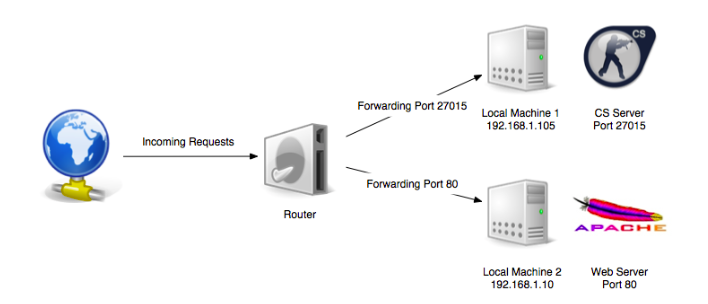
\includegraphics[width=10cm]{port.png}\\


\end{document}


















